\begin{figure*}[!hbtp]
  \centering

  \subfloat{
    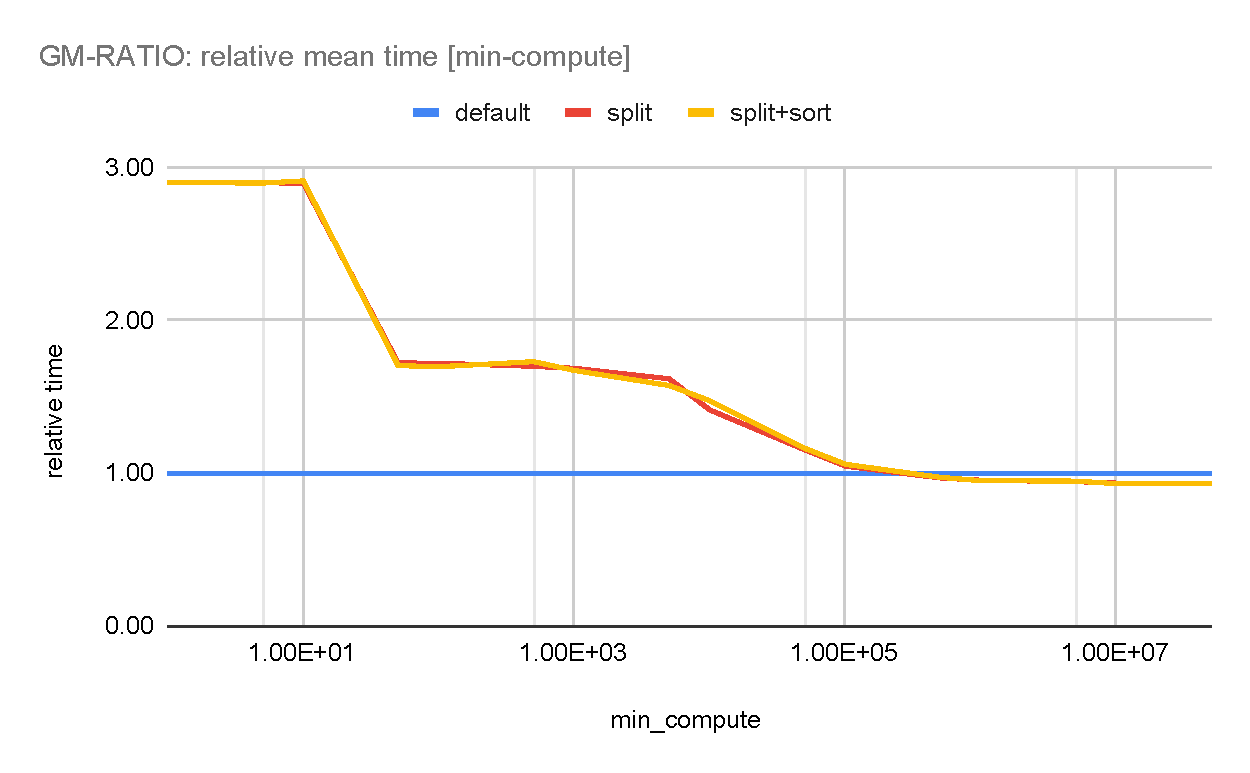
\includegraphics[width=0.48\textwidth]{out/pr-cuda-opt-s-rtime.pdf}
    \label{fig:pr-cuda-opt-s-rtime}
  }
  \subfloat{
    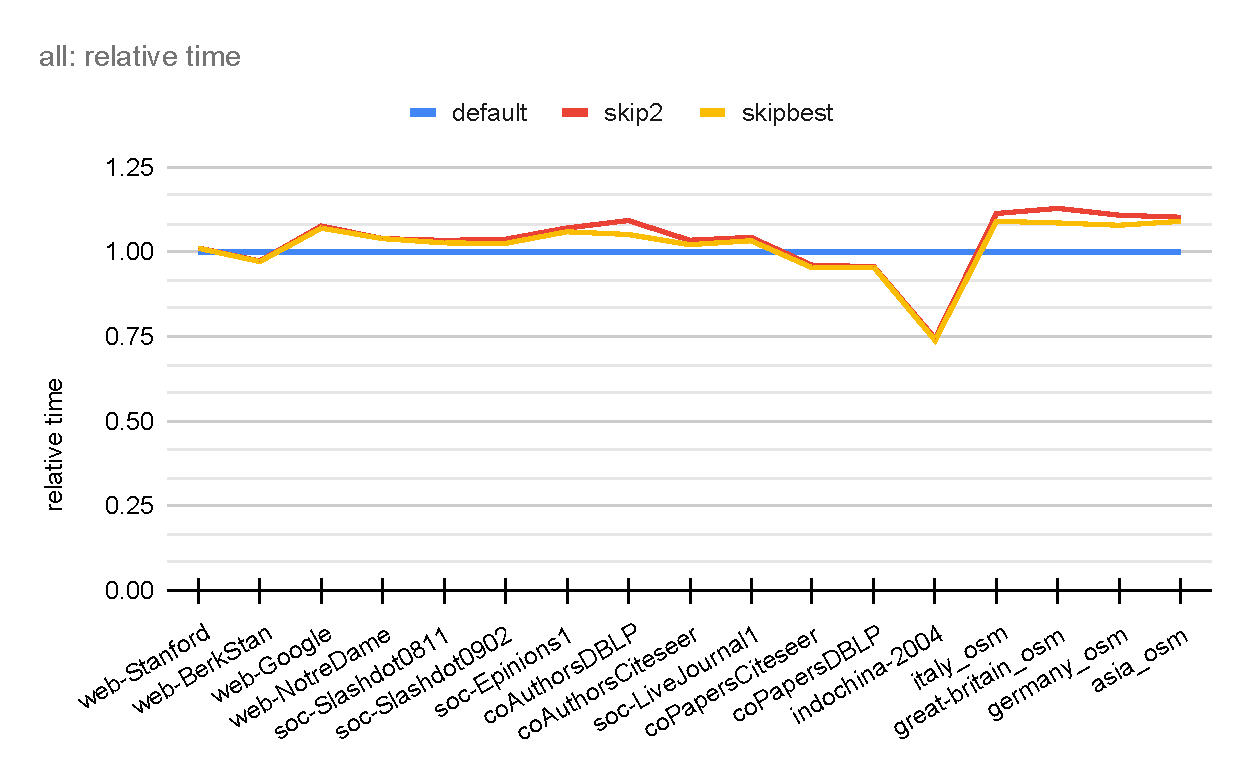
\includegraphics[width=0.48\textwidth]{out/pr-cuda-opt-i-rtime.pdf}
    \label{fig:pr-cuda-opt-i-rtime}
  }

  \caption{\textbf{Left:} Relative GM of time taken on all graphs for switched thread/block-per-vertex CUDA-based (GPU) static PageRank computation with the following algorithmic optimizations: no optimization (default), split vertices by components (split), and split vertices by components with each component sorted in topological order of its block-graph  (split+sort). This is relative to no optimization, with min. compute size ranging from 1 to 5×107. \textbf{Right:} Rel. time taken for switched thread/block-per-vertex CUDA-based (GPU) static PageRank computation with the following algorithmic optimizations: no optimization (default), skip all in-identicals (skip2), and skip in-identicals of best min. size  (skipbest). The ratio is obtained with respect to no optimization. This is done on 5 web graphs, 4 social networks, 4 collaboration networks, and 4 road networks.}
  \label{fig:pr-cuda-opt-si}
\end{figure*}
